\section{Evaluation}
\label{sec:eval}

% VALUE: what the evaluation establishes, then the order: the composer's reorder shortens prefill on five LLMs against the alternated baseline, the loop pass shortens decode, the event model chooses among schedules within a few percent; then end-to-end, sources, accuracy and bound, fidelity and reach, overheads
% DECISION: no question list at the head of the evaluation (contract: 2 of 19 sampled MLSys papers use one); subsections have noun titles and each opens with its finding.
In this section, we show that OPCORD's reorder across column groups shortens prefill on five LLMs, that its renaming shortens decode, and that the event model makes the choices that produce these gains.
After the setup, we report end-to-end latency, the sources of the gains, the event model's accuracy and the distance to the bound, the method's fidelity and reach, and its overheads.

\subsection{Experimental Setup}
\label{subsec:setup}

% VALUE: the platform and its power state, the software, the designs, and the five LLMs (one per class of edge LLM)
We measure on a GMKtec NucBox EVO-X2, whose AMD Ryzen\texttrademark{} AI Max+ 395 processor carries an XDNA~2 NPU of 8 columns of 4 compute tiles and 64\,GB of shared memory, under Linux~7.0 with the amdxdna driver, XRT~2.25.0~\citep{xdna-driver,xrt-repo}, and NPU firmware 1.1.2.65 in performance mode.
We rewrite MLIR-AIR's fused prefill and fused decode~\citep{wang2026mlirair}, compiled with MLIR-AIE~\citep{mlir-aie-repo}, for five LLMs with 4-bit weights, one per class of edge LLM: the dense Llama-3.2-1B~\citep{meta2024llama32}, Qwen3-4B~\citep{yang2025qwen3}, and Llama-3.1-8B, together with Gemma3-4B, which uses sliding-window attention, and LFM2-1.2B, which has convolution layers.
% SOURCE: machine files read 2026-10-14/15: uname -r 7.0.0-34-generic; amdxdna 2.25.0_20260922 (DKMS, 31c01f2019e7); XRT 2.25.0 (3923b2b5be55); NPU firmware 1.1.2.65 (sysfs fw_version); BIOS EVO-X2 1.12; NPU power mode performance, CPU EPP and governor performance (lab-prefill-overlap (11), lab-split-sweep (9)).
% SOURCE: mlir-air a3e26261 (llms/shared/fused_prefill, fused_decode); mlir_aie wheel 1.4.5.dev22+g35fa6b1; weights FastFlowLM/Qwen3-4B-NPU2 rev 07651f11cac7, the Llama-3.2-1B q4nx bundle, FastFlowLM/Llama-3.1-8B-NPU2 rev 52700648, all sha256-verified (lab-prefill-overlap (23), lab-split-sweep (10)).
% DECISION: the BIOS power mode cannot be read from the OS; add it once the author records it.

% VALUE: the workloads, placed on the step distribution of real coding agents, with the context limit and why the longest decode context is 32,512
Prompts computed from scratch have 2{,}048 or 4{,}096 tokens, and appends add 2{,}048 or 4{,}096 tokens to cached contexts of 2{,}048 to 16{,}384 tokens.
A turn appends 512 to 4{,}096 tokens to a context of up to 28{,}672 and decodes 250, which spans the 25th to the 90th percentile of new tokens per step in coding-agent traces~\citep{zhu2026tracelab}.
Our contexts stop at the 32{,}768-token window of the decode designs we build, below those traces' median prefix of 119K tokens.
% SOURCE: TraceLab Table 8: append tokens P25 / P50 / P90 = 384 / 857 / 5,342 (Claude) and 406 / 886 / 8,310 (Codex); output P50 252 / 184; Section 1: median prefix 119K, append 875, output 214 (PDF read 2026-10-15).
% SOURCE: append grids: 4,096 onto 4,096 or 16,384 (the split sweep); 4,096 onto 2,048 or 8,192 and 2,048 onto 12,288 (Table append, the event model and the bound); turns 512 / 1,024 / 4,096 onto 4,096 / 16,384 / 28,672 plus 250 decoded tokens. Turn cells excluded before running: 28,672 + 4,096 (L + N + 250 > 32,768, the 1B decode window); Qwen3-4B at 28,672 (its decode KV buffer passes the 4 GiB shim-offset bound) (vault lab-agent-step (5)). Full grid statement: Appendix percell.
% DECISION: the append grid of Table append (cached contexts 2,048 / 8,192 / 12,288) and the turn grid (4,096 / 16,384 / 28,672) are disjoint, and no turn cell carries an event-model prediction; each number names its grid where it is quoted.
% COMMENT: being extended per D19c (decisions log, 2026-10-22): the 1B to its native window, the 8B and Qwen3-4B past the 4 GiB a single cache buffer can address by splitting it. The earlier clause "an edge model's window" was wrong: 32,768 is our build window, not the models'.

% VALUE: the baselines: the existing program on its default split; the alternated baseline with the obvious hand fix, each side at its own faster split, so prefill gains are over a program that already has that fix; decode and turns name their own baselines; FastFlowLM as an absolute reference only
Every result compares against the fastest existing schedule we measured for its design.
For prefill, that is the existing program with attention's two columns alternated by hand, which removes the one false dependence visible without reading the command stream and which we call the \emph{alternated baseline}, with it and OPCORD each on its own faster split.
For decode, it is the unmodified decode design, and for turns, the existing program on its faster split.
FastFlowLM~\citep{fastflowlm-repo}, which ships hand-tuned designs for this device, gives an absolute reference on the same weights.
% DECISION: the alternated baseline is ours to construct and is described as such; it uses the same configuration, kernels, and weights as the composed schedules. FastFlowLM is a reference point, never a speedup claim (D14 MUST 5; ruling of 2026-10-21).

% VALUE: correctness gates, the one LLM whose reference check limits what we report, the metrics, and the run protocol with the batch rule; defaults stated once
Every run's logits are bit-identical to the existing program's, every append's to a full prefill of the whole prompt, and the kernel log stays free of driver and IOMMU messages.
Gemma3-4B's existing prefill already changes the fifth decoded token against a floating-point reference, so we report its prefill but no turn (Appendix~\ref{app:gemma-gate}).
TTFT is the wall time of the prefill call, the time per token is the inverse of the decode rate over 250 greedy tokens, and a turn is an append and 250 decoded tokens, excluding the handoff of the KV cache that both sides pay and the composer's planning, which Section~\ref{subsec:overheads} prices.
We report medians of five runs for prefill and three for decode and turns, after a warm run and in rotated order.
Because the DRAM read cap varies by up to 12\% between batches, every ratio compares runs from one batch.
% SOURCE: run counts: five prefill, three decode and turns, one warm run; Llama-3.1-8B decode five, paired, over 256 tokens (lab-decode-long-context (44)).
% VERIFY (re-run): five and three are the protocol every campaign quoted here was run under, except Gemma3-4B's
% first split sweep, whose two-rep medians were superseded by a five-rep rerun agreeing within 0.08% (Appendix~E),
% and the decode fit in Section 2, which is a median of three. The full re-run puts every cell on one count.
% SOURCE: lock = flock ~/.local/state/npu.lock; brackets = 1x1 and 8x2 DRAM reads of 256 MiB, the dispatch floor, load, NPU mode, EPP, governor; 8x2 cap 49.9-55.7 GB/s over the batches, 55.7 / 49.9 = 1.116 (lab-prefill-device (1), lab-prefill-overlap (2), (11), lab-split-sweep (4)-(5), lab-agent-step (2)).
% DECISION: the run count is fixed at the results freeze; a count that differs by comparison is stated where it applies.
% DECISION: a turn EXCLUDES the KV handoff on BOTH models (metric decision, plan c72f5ce); the handoff is priced in the appendix, not in the turn paragraph (author, 2026-10-23: details out of the body); was: the turn paragraph gives the 1B's with-handoff range so a reader can deflate the ratios.

\subsection{End-to-End Latency}
\label{subsec:e2e}

% VALUE: OPCORD shortens prefill on every LLM against the alternated baseline, each side at its faster split, from scratch and on appends, with bit-identical outputs; the gain is smallest where a short append meets a long context, which points to the GEMM work the reorder can run beside attention
OPCORD shortens prefill on all five LLMs, and decode and whole agent turns on Llama-3.2-1B and Qwen3-4B, with outputs bit-identical to the existing program's.
Against the alternated baseline, OPCORD lowers TTFT by $1.14$--$1.46\times$ from scratch and by $1.19$--$1.51\times$ on appends to a cached context (Table~\ref{tab:append}).
On every LLM the gain is smallest on the 2{,}048-token append to a 12{,}288-token context, whose new tokens bring the least GEMM work while attending to the most cached ones, which indicates that the reorder's gain follows the GEMM work it can run beside attention.
% SOURCE: from scratch, each side on its own faster split against the alternated baseline: Llama-3.2-1B 1.25 / 1.45, Qwen3-4B 1.27 / 1.46 at 2,048 / 4,096 (vault lab-split-sweep (18), amd-npu ba9f6f8); Llama-3.1-8B 1.14 / 1.27 (lab-split-sweep (20)); Gemma3-4B 1.212 / 1.259 (lab-split-sweep (21)-(22), amd-npu 08a56cd; S4 rerun at 5 reps within 0.08%, lab-split-sweep (23), amd-npu e9e386e); LFM2-1.2B 1.145 / 1.215 against min(shipped S2, shipped + Ar S2, shipped S4, shipped S1) (lab-split-sweep (28), amd-npu e695d3dd). Range over the five LLMs 1.14-1.46.
% SOURCE: appends, re-derived from amd-npu 78ec55b7 prefill-overlap/cp-predict/score-2026-10-21.json through Table append: gains 1.197-1.511 over the twelve cells, smallest per LLM at 12,288 + 2,048 (1B 1.205, Qwen3-4B 1.216, Gemma3-4B 1.197, 8B 1.364). LFM2-1.2B appends 1.217 / 1.194 at 4,096 + 4,096 / 16,384 + 4,096 against the same strongest base (lab-split-sweep (28)), with each append identical to a full prefill including the carried convolution state.
% SOURCE: the split-sweep appends of the other four LLMs (4,096 + 4,096 and 16,384 + 4,096, against the same alternated baseline): 1B 1.46 / 1.33, Qwen3-4B 1.46 / 1.33, 8B 1.48 / 1.49, Gemma3-4B 1.291 / 1.172 (lab-split-sweep (18), (20), (21)-(23)); not quoted as a range because Table append is the fuller append record; Section 7.3 uses them per split.
% DECISION: one range per regime. From scratch, the split sweep is the only record and covers all five LLMs; on appends, Table append (12 cells, four LLMs, three splits, three arms) is the fullest, and LFM2's two appends are named apart because they sit on the other grid.
% VALUE: the append phase in absolute times, one row per model and cell, so a reader sees what the gains are of and
% how far the bound still is. Per-phase tables rather than one combined table: the grids differ by phase (appends
% are scored on L in {2,048, 8,192, 12,288}, decode on context length, turns on a third grid), and one table over
% three grids would imply cells that were never run.
% SOURCE: every number re-derived in this workspace from the committed campaign score (amd-npu 78ec55b7
% prefill-overlap/cp-predict/score-2026-10-21.json, scorer cp_score.py 86ba24b6, holds fd6e6c7b committed before
% reading). Baseline = the shipped program with attention's columns alternated (shipar), at its own faster split
% over the splits measured for that model; composed = the composer at its own faster split; bound = the composed
% arm's measurement divided by the B2 ratio the scorer recorded, so it is the bound at the composed schedule's
% split and not the smallest bound over splits that Section 5.7's gap analysis uses.
% DECISION: the shipped arm without the hand alternation is not a column. It differs from the baseline by under
% 0.1% in eleven of these twelve cells, because the composer's split is S4 on nine of them and on S4 attention
% already has two segments per column, so alternating changes nothing. The one exception, Llama-3.1-8B at
% 2,048 + 4,096, is stated in the text.
% DECISION: the model is a spanning row rather than a column, so the table fits one column at \small; a
% full-width table* for twelve short rows would cost more page than the phase is worth.
\begin{table}[t]
\caption{Time from a tool result to the first new token, on appends of $N$ tokens to a cached context of $L$. Each arm is at its own faster split, and $S_k$ is the split the composed schedule takes, $k$ being attention's columns. The baseline is the shipped program with attention's two columns alternated by hand. The bound comes from the same per-operator probes, at the composed schedule's split.}
\label{tab:append}
\vskip 0.1in
\centering
\small
\begin{tabular}{lcrrrr}
\toprule
$L + N$ & Split & Base & Comp. & Bound & Gain \\
        &       & (ms) & (ms)  & (ms)  &      \\
\midrule
\multicolumn{6}{l}{\textit{Llama-3.2-1B}} \\
2{,}048 + 4{,}096 & $S_4$ & 1{,}906 & 1{,}387 & 1{,}160 & $1.37\times$ \\
8{,}192 + 4{,}096 & $S_4$ & 2{,}769 & 1{,}852 & 1{,}496 & $1.50\times$ \\
12{,}288 + 2{,}048 & $S_4$ & 1{,}613 & 1{,}339 & 977 & $1.20\times$ \\
\addlinespace[2pt]
\multicolumn{6}{l}{\textit{Qwen3-4B}} \\
2{,}048 + 4{,}096 & $S_4$ & 6{,}612 & 4{,}927 & 4{,}227 & $1.34\times$ \\
8{,}192 + 4{,}096 & $S_4$ & 9{,}685 & 6{,}408 & 5{,}301 & $1.51\times$ \\
12{,}288 + 2{,}048 & $S_4$ & 5{,}630 & 4{,}631 & 3{,}448 & $1.22\times$ \\
\addlinespace[2pt]
\multicolumn{6}{l}{\textit{Gemma3-4B}} \\
2{,}048 + 4{,}096 & $S_2$ & 4{,}221 & 3{,}260 & 2{,}619 & $1.29\times$ \\
8{,}192 + 4{,}096 & $S_2$ & 4{,}854 & 3{,}864 & 2{,}619 & $1.26\times$ \\
12{,}288 + 2{,}048 & $S_2$ & 2{,}575 & 2{,}151 & 1{,}319 & $1.20\times$ \\
\addlinespace[2pt]
\multicolumn{6}{l}{\textit{Llama-3.1-8B}} \\
2{,}048 + 4{,}096 & $S_2$ & 9{,}625 & 6{,}566 & 5{,}599 & $1.47\times$ \\
8{,}192 + 4{,}096 & $S_4$ & 12{,}730 & 9{,}233 & 7{,}917 & $1.38\times$ \\
12{,}288 + 2{,}048 & $S_4$ & 7{,}064 & 5{,}177 & 3{,}968 & $1.36\times$ \\
\bottomrule
\end{tabular}
\vskip -0.1in
\end{table}


% VALUE: FastFlowLM as an absolute reference: the composed schedule is below FastFlowLM in every configuration, and the existing program it rewrites is already close to it, so the gains are not measured against a slow baseline; not like for like
For an absolute reference, the composed schedule's TTFT is $1.31$--$1.86\times$ below FastFlowLM's on the same weights across three LLMs, from scratch and on appends.
The existing program alone takes $0.67$--$1.11\times$ FastFlowLM's time, so our gains are not measured against a slow baseline.
The two stacks differ in kernels and quantization, so this is a reference point rather than a like-for-like speedup (Appendix~\ref{app:flm}).
% SOURCE: FastFlowLM v1.0.8 unmodified, flm serve -c 32768 --pmode performance, TTFT = the server's prefill_duration_ttft, median of 5 rotated reps (client times 5-22 ms above it), token targets hit exactly 5/5 per cell, cached_tokens 0 on every scratch and turn-1 prompt, power mode read back performance, brackets 13.35-13.70 GB/s (1x1): 1B 989.9 / 1,818.6 / 4,508.4 ms, Qwen3-4B 3,190.6 / 5,988.0 / 13,563.9, Llama-3.1-8B 4,297.3 / 8,051.6 / 14,739.7 at scratch 2k / scratch 4k / 16k + 4k; FastFlowLM over the existing program 1.49 / 1.13 / 1.15 (1B), 1.42 / 1.09 / 0.98 (Qwen3-4B), 1.24 / 1.03 / 0.90 (8B), and over the composer 1.86 / 1.64 / 1.53, 1.81 / 1.59 / 1.31, 1.42 / 1.31 / 1.34; the 8B served at its full 32,768-token capacity (vault lab-flm-practice (6), amd-npu 77b04b56, beeb6ce3, d426519d, ee472858).
% SOURCE: not in the range: FastFlowLM gemma3:4b, prefill_duration_ttft median of 5, 2,587.9 / 4,560.0 / 5,215.9 ms at 2k / 4k / 16k + 4k against MLIR-AIR's best existing 1,857.1 / 3,898.7 / 5,382.1 and best composer 1,531.9 / 3,096.2 / 4,592.9 from (22) / (23), measured in a different batch (lab-flm-practice (15), amd-npu 2c79ecf5); that hold ran beside an orphaned host process and its host-timed numbers are flagged (decisions log, host-load disclosure, 2026-10-23). Including it would make the range 1.14-1.86x.
% SOURCE: FastFlowLM chunks prefill at up to 4,096 tokens, from its server log (1 chunk in every measured cell), against the existing MLIR-AIR prefill's 128 (vault lab-flm-practice (6)).
% DECISION: this is a reference point, never worded as a speedup over FastFlowLM (D14's reviews, MUST 5; ruling of 2026-10-21). The appendix lists the inequalities.

% VALUE: decode: renaming the KV loop lowers time per token, against the unmodified decode design, by a factor that grows with the context and with the ratio of serialized compute to transfer per position; absolute rates for readers who compare stacks; after renaming the 1B's loop is bound by its value kernel; level with FastFlowLM's hand-tuned time at long context, behind at short context by an LM-head gap renaming does not touch
\label{subsec:decode-eval}
Because our loop pass lets each block's transfer overlap the compute on the previous block, the decode gain grows with the context, as attention's share of each token does (Figure~\ref{fig:decode}).
At 16{,}384 tokens, the renamed design lowers the time per token against the unmodified decode design by $1.27\times$ on Llama-3.2-1B and $1.16\times$ on Qwen3-4B, decoding 35.6 tokens per second against 28.1 and 9.8 against 8.5, and by up to $1.39\times$ at 32{,}512 tokens.
The gain is smaller on Qwen3-4B because its serialized compute per position is 0.34 of its transfer, against 0.71 on the 1B.
At this context, the renamed design matches the time per token of FastFlowLM's hand-tuned decode within 2\%, where the existing design takes $1.18$--$1.29\times$ as long.
% SOURCE: the R arm (the loop pass through the compiler hook) of the gate run, vault lab-decode-long-context (22): Llama-3.2-1B 35.621 -> 28.072 ms (1.269x) at P = 16,384 and 54.160 -> 38.938 ms (1.391x) at 32,512 (1.394x at its parity twin 32,517), slope 0.683 us per position against a MEASURED transfer-only 0.677 (+0.9%); Qwen3-4B 118.172 -> 101.839 ms (1.160x) at 16,384 and 168.781 -> 140.058 ms (1.205x) at 28,800, slope 3.099 against a DERIVED transfer-only 3.047; tokens and every step's logits bit-identical across the baseline, the hand edit and R at every point (amd-npu a6bc94b6 gate-1b.json sha256 36472797..., 455740b1 gate-qwen.json sha256 38e750a2...).
% SOURCE: tokens per second = 1000 / ms per token from the same gate run: 1B 28.07 -> 35.62 tok/s, Qwen3-4B 8.46 -> 9.82 tok/s at P = 16,384.
% SOURCE: serialized compute over transfer per position 0.34 (Qwen3-4B) and 0.71 (1B) (lab-decode-long-context (14)).
% SOURCE: at a 16,384-token context the renamed design takes 1.014x FastFlowLM's time per token on Llama-3.2-1B (28.07 / 27.68 ms) and 1.013x on Qwen3-4B (101.84 / 100.52 ms), our points 3 and 19 positions from FastFlowLM's; the existing design 35.62 / 27.68 = 1.287x and 118.17 / 100.52 = 1.176x (figs/data/decode-1b.json, decode-qwen.json; FastFlowLM amd-npu 86ef630 flm-practice/results/2026-10-19/results.json).
% DECISION: quote the R arm, which is the pass the paper ships, and say so where a figure or a number names "the renamed loop". The earlier W2 runs (lab-decode-long-context (13) and (15), amd-npu aab2aae / 320d2d3) give 1.274 / 1.366 and 1.17 / 1.21 with a 1B slope 5% above transfer; those are a different run and must not be mixed with (22)'s numbers in one sentence.
% DECISION: the absolute decode rates stay in the text (author, 2026-10-23) as a reference magnitude for readers who compare engines in tokens per second; they are the one exception to relative numbers in this subsection.

\begin{figure}[t]
    \centering
    % VALUE: the decode result as a curve rather than a table, because what the renaming changes is the slope per
    % position and not a single cell: the baseline's cost per position is the transfer plus the compute it waits
    % for, and the renamed loop's is the transfer alone.
    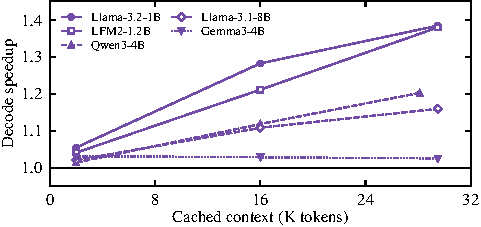
\includegraphics{fig/decode.pdf}
    \caption{Decode time per token against the length of the cached context, for the existing design and after our loop pass renames the keys, values, and scores into rings. Each point is the median of three runs of 250 tokens, and every step's logits are bit-identical between the two designs at every point. The annotation on each panel is the fitted cost per decoded position.}
    \label{fig:decode}
\end{figure}
% SOURCE: figs/data/decode-1b.json and decode-qwen.json, byte copies of amd-npu a6bc94b6 gate-R/1b-2026-10-21/gate-1b.json and 455740b1 gate-R/qwen-2026-10-21/gate-qwen.json; the figure plots the census (baseline) and R (our pass) arms and drops the 32,517 reproduction point, which repeats 32,512.
% DECISION: the event model's decode prediction and the cap-bounded estimate are not plotted. Neither is in these two records, and adding a line the data file does not carry would make the figure unreproducible from figs/data.

% VALUE: whole turns, against the existing program on its faster split: the gain rises with the cached context; at the traces' most common step it is moderate, and larger against the existing program on its default split; decode carries most of the gain and the composed prefill adds only at the largest steps; decode runs the hand renaming the pass matches; the handoff both sides pay, quoted so a reader can deflate the ratios
\label{subsec:turns}
The gain on a whole turn rises with the cached context.
Against the existing program on its faster split, OPCORD shortens a turn by $1.06$--$1.23\times$ at a 4{,}096-token context and $1.15$--$1.32\times$ at 16{,}384 on both LLMs, and by $1.33$--$1.34\times$ at 28{,}672 on the 1B, the one LLM we measure there (Figure~\ref{fig:turns}).
At the traces' most common step, about a thousand new tokens onto 16{,}384, a turn is $1.15$--$1.26\times$ shorter.
Decode carries most of the gain, since on renamed decode the composed prefill adds $1.09$--$1.10\times$ to steps of 4{,}096 tokens and nothing measurable to steps of up to 1{,}024.
In these turns, decode runs the renaming applied by hand, which our loop pass matches within 1\%.
% SOURCE: the composer over renamed decode on the existing S4 prefill: 1.088-1.098x at N = 4k, 0.993-1.004x at N <= 1k on both models (vault lab-agent-step (8), (10); amd-npu c61445d, 171082f).
% SOURCE: re-derived from the committed per-rep files (amd-npu c61445da turn-w3-1b.json, 171082f6 turn-w3-qwen.json), turn = median(append) + median(decode), best-vs-best = min over the two existing splits / min over the two composed ones, no handoff: Llama-3.2-1B 4k+512 1.096, 4k+1k 1.113, 4k+4k 1.229, 16k+512 1.256, 16k+1k 1.255, 16k+4k 1.316, 28k+512 1.336, 28k+1k 1.326; Qwen3-4B 4k+512 1.060, 4k+1k 1.076, 4k+4k 1.183, 16k+512 1.146, 16k+1k 1.150, 16k+4k 1.218. Against the existing default (its S2 with the unrenamed decode): 1B 1.118 / 1.157 / 1.460 / 1.374 / 1.500 / 2.173 / 1.435 / 1.513; Qwen 1.084 / 1.128 / 1.519 / 1.216 / 1.284 / 1.663; at 16,384 + 1,024 1.500 and 1.284.
% SOURCE: the turn harness runs census vs (c) decode (vault lab-agent-step (8), (10)); the loop pass's per-token time within 0.992-1.004 of (c) on the 1B and Qwen3-4B (lab-decode-long-context (22)).
% SOURCE: the 1B WITH its steady handoff, best-vs-best 1.088 / 1.104 / 1.215 / 1.235 / 1.236 / 1.295 / 1.307 / 1.300; handoff in the clean state 6.2-8.6% of the turn on the 1B and 3.4-8.2% on Qwen3-4B's clean cells (computed from the same per-rep files; the composed arm's smallest handoff per cell against its own turn).
% DECISION: 28,672 is quoted on Llama-3.2-1B alone, since Qwen3-4B has no cell there; the sentence says "the one LLM we measure there" rather than implying both.
% DECISION: the 1B's 16,384 + 4,096 existing-S2 run ran in the existing program's usual long-context mode (append 12.8-13.1 s), which D23 classes as representative rather than anomalous; its best-vs-best ratio takes the S4 arm and is unaffected. Qwen3-4B's 16k with-handoff ratios are not quoted (the handoff's page-fault state, Appendix handoff).

\begin{figure}[t]
    \centering
    % VALUE: the turn speedup over the step size and the cached context, placed on the traces' step distribution
    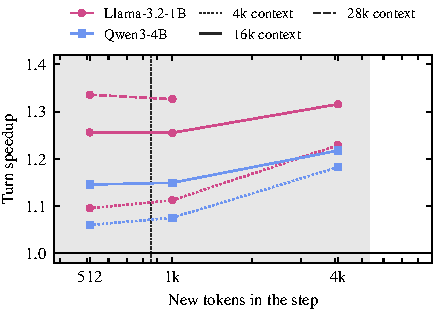
\includegraphics{fig/turns.pdf}
    \caption{Whole-turn speedup against the existing program on the faster of its two-column and four-column splits, by the number of new tokens in the step and the length of the cached context. A turn is its append and 250 decoded tokens, without the handoff of the KV cache. The shaded band spans the 25th to the 90th percentile of the new tokens per step in coding-agent traces and the dotted line is their median~\citep{zhu2026tracelab}.}
    \label{fig:turns}
\end{figure}

\subsection{Sources of the Gains}
\label{subsec:ablation}

% VALUE: what each part contributes: every prefill gain over the alternated baseline is the composer's reorder across column groups, which nothing hand-written or shipped does; the stream pass reproduces the alternation the baseline carries, so its gain over it is zero by construction, and the loop pass's decode renaming is the hand edit experts make, reaching FastFlowLM's time per token at long contexts; the passes' value is reach (§7.5, judged, not gains); the event model contributes the choices (§7.4)
Every prefill gain over the alternated baseline comes from the composer's reorder across column groups, which no hand-written or shipped design performs.
The two passes automate inside the compiler what experts do by hand, so their value is reach, applying an expert's edit legally to designs nobody tuned (Section~\ref{subsec:fidelity}).
The stream pass reproduces the hand alternation that the alternated baseline already carries, and the loop pass's renaming matches FastFlowLM's hand-tuned decode (Section~\ref{subsec:e2e}).
The event model contributes the choices, namely the split per regime and whether a removal pays (Section~\ref{subsec:accuracy}).

% VALUE: what contributes nothing to the prefill gain: packing alone, and the split (credited to neither side)
None of the gain comes from packing alone (Section~\ref{subsec:semantics}), and we credit the split to neither side, because the existing program's faster split flips with the regime as ours does (Appendix~\ref{app:split-first}).
% SOURCE: 16k + 4k append, composed on S4 vs composed on S2: Llama-3.2-1B 5,493.0 -> 2,950.8 ms (1.86x), Qwen3-4B 19,332.6 -> 10,342.7 ms (1.87x) (vault lab-split-sweep (4)-(5)); this is the split's own gain, credited to the regime and not quoted here.
% SOURCE: the shipped + Ar faster split equals the composer's faster split in 8 of 8 W1 cells (vault lab-split-sweep (18)) and 11 of 12 Table append cells (amd-npu 78ec55b7 E1 calls, the twelfth a near tie); Llama-3.1-8B 4k + 4k is the one other disagreement (Appendix split-first). Corrected 2026-10-22 (D19 convergence point 4).
% SOURCE: R-ship (the composed schedule at the existing program's per-chunk naming) equals the composer with rings within 0.1% (0.99996-1.00074, amd-npu 71081d1).
% DECISION: the split is a finding priced by the event model, not a removal over a baseline at its own faster split (D19 point 4); the reorder's gain is always quoted with each side at its own faster split.

% VALUE: the prefill reorder has two parts that the splits separate: within attention's two columns (the alternation the stream pass emits, measured against the existing program) and across column groups (the composer); at four columns the existing stream already alternates, so only the cross-group part remains; the within-operator share grows with the context while the cross-group share shrinks as attention takes over
In prefill, the reorder has one part between attention's two columns and one across column groups (Figure~\ref{fig:schedules}).
At the four-column split, the existing attention stream already issues two segments per column before it waits, so the hand alternation changes nothing there (Appendix~\ref{app:percell}).
The reorder across groups alone then gains $1.11$--$1.22\times$ from scratch and $1.33$--$1.46\times$ on appends on Llama-3.2-1B and Qwen3-4B, and on Gemma3-4B, whose attention stream has no wait to alternate at any split, it carries the whole gain.
At the two-column split, the alternation that the stream pass emits gains $1.12$--$1.42\times$ over the existing program and leaves $1.13$--$1.46\times$ to the reorder across groups.
The two parts move in opposite directions with the context, and on the append to 16{,}384 tokens the alternation gives $1.42\times$ and the reorder across groups $1.13\times$, since attention then holds most of the time.
% SOURCE: vault lab-split-sweep (22), medians of 5, the four cells being scratch 2,048 / scratch 4,096 / 4,096 + 4,096 / 16,384 + 4,096. At S4 shipped + Ar equals shipped within 0.0%, so composer over shipped is the cross-group reorder alone: 1B 1.13 / 1.22 / 1.46 / 1.33, Qwen 1.11 / 1.19 / 1.46 / 1.33. At S2 the order's gain splits into within-operator (shipped -> shipped + Ar) 1B 1.12 / 1.19 / 1.34 / 1.42, Qwen 1.13 / 1.20 / 1.37 / 1.42, and across-operator (shipped + Ar -> composer) 1B 1.25 / 1.45 / 1.37 / 1.13, Qwen 1.27 / 1.46 / 1.36 / 1.13.
% SOURCE: the segment counts are read from the existing attention streams at each split by our own analysis, and the equality is measured: at S4 shipped + Ar equals shipped within 0.1% on every cell of every model (vault lab-split-sweep (22)).
% DECISION: the 1.33x at 16,384 + 4,096 here is prefill TTFT and must not be conflated with a whole-turn ratio at a 28,672-token context.
% DECISION: the alternation is what the stream pass emits byte-identically on all 42 attention streams (Section 6); the text credits it as the within-operator removal, never as something the pass discovers.

\begin{figure}[t]
    \centering
    % VALUE: the decomposition in one picture: the composed schedule is below both existing schedules at every split of every
    % LLM, the hand alternation closes part of that distance only where attention has a wait to remove, and
    % which split is fastest is a property of the LLM rather than of the regime.
    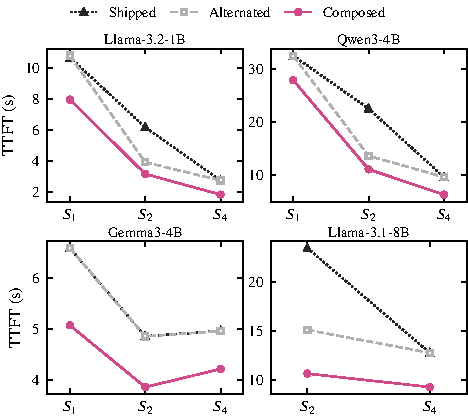
\includegraphics{fig/schedules.pdf}
    \caption{Time to the first new token by split, for the existing schedule, the existing schedule with attention's columns alternated by hand, and the composed schedule, on an append of 4{,}096 tokens to an 8{,}192-token context. $S_k$ gives attention $k$ of the eight columns. The existing and alternated schedules coincide wherever attention has no wait to alternate away, which is every split on Gemma3-4B and the four-column split on the others. Llama-3.1-8B is built on two splits only.}
    \label{fig:schedules}
\end{figure}
% SOURCE: figs/data/accuracy.json, the claimed and reported arms at cell append:8192:4096; the packed-into-one-command arm is not plotted because the only whole-model measurement of it predates the composer this paper evaluates, and Section~\ref{subsec:semantics} establishes at operator-pair scale that packing alone creates no overlap.


% VALUE: decode's gain needs the whole cycle renamed: keys and values alone gain nothing while the score buffer closes the cycle
In decode, renaming the keys and values alone, as a production mapping of another LLM does by hand~\citep{du2026gemma3}, is worth 0.3\%, because the shared score buffer still closes the loop's critical cycle, as the condition of Section~\ref{subsec:removal} requires.
% SOURCE: keys and values renamed with the existing score buffer kept: 1.002x (16,384) and 1.003x (32,512), tokens and logits bit-identical (vault lab-decode-long-context (28); amd-npu d8f0bd4c, score 5e1017a5); all three renamed (the loop pass): 1.269x / 1.391x (lab-decode-long-context (22)).

% VALUE: where removal does not pay, each with its measured reason: short appends where the composed pipeline is mostly fill and drain (the event model prices it right, and the turn still gains), and Llama-3.1-8B where both phases already read near the DRAM cap so only serialized compute remains to hide
Removal does not pay where a measured term leaves it nothing to hide.
At 512-token appends, the composed prefill runs at $0.88$--$0.93\times$ the existing order's speed, because with four chunks per layer its pipeline of in-flight commands is mostly fill and drain, which the event model prices correctly at all three contexts.
Llama-3.1-8B gains least from scratch, because its composed prefill already reads 93--96\% of the read cap.
% SOURCE: the 512-token appends, existing S4 faster at 0.88-0.93x (vault lab-agent-step (8), (10)); computed after the turns were measured, with the model unchanged (amd-npu e30be08 adds cell selection only; two earlier cells reproduce bit-identically): the model prices the existing S4 order below the composed one, 249.9 / 469.7 / 689.4 vs 294.7 / 513.6 / 732.4 ms at 4k / 16k / 28k (measured 265.0 / 482.1 / 699.7 vs 300.6 / 521.3 / 754.3), and the faster S4 order on 14/14 turn cells; at 1k appends its margin is 0.2-0.3%, inside its error, and choosing by it costs at most 23 ms of a turn (vault lab-agent-step (11), amd-npu 9d4f63f). Fill and drain: lab-agent-step (11), Section~\ref{subsec:removal}. Turn at 512-token appends, best-vs-best 1B 1.096 / 1.256 / 1.336, Qwen3-4B 1.060 / 1.146.
% SOURCE: 8B composer read rate over TTFT including host time, 51.5 GB/s at scratch 4,096 (its GEMM group 48.2) and 50.8 at scratch 2,048, against the 53.9-55.3 GB/s cap; bytes from the TXN BD chains over the measured TTFT (amd-npu 71901c50; vault lab-metric-fields (1), amendment 1).
% SOURCE: amd-npu 25f6adde decode-rename/w2c-8b-run-2026-10-22/score.json (vault lab-decode-long-context (44)). 16,384: baseline 192.617 ms/token, renamed 178.660, r median 1.0785 [1.0738, 1.0839], no-chain ceiling 1.0855. 30,720: 204.572 and 179.359, r 1.1397 [1.1356, 1.1511], ceiling 1.1597. Tokens and every step's logits identical across arms and repetitions. The partial arm on the same baseline and cells is 0.990x (lab-decode-long-context (19)).
% DECISION: the 512-token result is stated as a pricing checked against the measurement, not as a choice the system made during the runs.
% DECISION: the 8B decode is quoted as the bound predicting a small gain, never as a disappointment; the hand edit is the arm measured on that LLM, and the loop pass's 8B build is bit-identical but untimed.

\subsection{Model Accuracy and the Bound}
\label{subsec:accuracy}

% VALUE: the event model names the faster split in every case and orders every clearly separated pair; it prices the composed schedule within a few percent, always slightly high, and the baselines slightly low, so it understates gains; its value over interpolation is coverage: it prices, without running it, any configuration within each operator's probed range
The event model names the faster split in all 36 cases, one per append configuration of Table~\ref{tab:append} and schedule, against 27 for the better rule that always answers with one split, and orders all 83 pairs of schedules whose times differ by at least 5\%.
It prices the composed schedule at its chosen split within a median 2.15\% and a maximum 7.31\%, always slightly high, and the baselines a median 2.2\% low.
% SOURCE: scorer cp_score.py 86ba24b6 unchanged, output amd-npu 78ec55b7 prefill-overlap/cp-predict/score-2026-10-21.json, holds fd6e6c7b committed before reading; re-derived from that file: E1 36/36, constant-rule patterns 27 and 25, 33/33 excluding near-ties; E2 83/83 at a 5% gap; E3 (the composer at the model's chosen split) median 2.146%, max 7.311% (Qwen3-4B 8k + 4k), every one an over-prediction (+0.04% to +7.3%); baseline arms under-predicted, median -2.2% shipped and -2.1% shipped + Ar over 33 each; interpolation 2.30% against 1.95% on its 10 cells; E4 measured - predicted = +0.085 / +0.118 / +0.057 / +0.018 / +0.090 / +0.037 / +0.048 / +0.042 / +0.030 / +0.006 / -0.001 / +0.053 (vault lab-split-sweep (27)).

% VALUE: pricing each configuration beats a regime rule because the faster split varies with the LLM, not only with the regime; the event model's error grows only on schedules it never chooses; on a fifth LLM whose layers are not all attention it still names the faster split and orders the pairs
Pricing each configuration matters because the faster split varies with the LLM as well as with the regime.
On these appends Llama-3.2-1B and Qwen3-4B want four attention columns in every configuration and Llama-3.1-8B in seven of nine, whereas Gemma3-4B wants two in seven of nine.
Its error grows only on schedules it never chooses, such as those on the one-column split.
On LFM2-1.2B, whose layers are not all attention, it names the faster split in 7 of 8 cases, where the one exception is a pair 0.1\% apart, and orders all 19 pairs that differ by more than 5\%, at a median error of 2.6\%.
% SOURCE: computed from the same scorer output: measured faster split over the 36 calls is S4 in 27 and S2 in 9; by model, 9/9 S4 on Llama-3.2-1B and on Qwen3-4B, 7 of 9 S2 on Gemma3-4B, 2 of 9 S2 on Llama-3.1-8B; constant rules score S4 27, S2 9, S1 0.
% SOURCE: other arms (lab-split-sweep (27)): S1 under-predicted to -38.5% (1B 12k + 2k, shipped and shipped + Ar), the composer on S1 to -31.8%; shipped on S2 -15.2% (8B 8k + 4k), -20.4% (1B 12k + 2k), -14.6% (Qwen3-4B 8k + 4k); none is ever the best split. The existing order's alternation ratio is lower at the 1B's mid-range chunks (0.41-0.57 against 0.66-0.68; lab-agent-step (4)), which the probes of a 2,048-token prompt do not see; no cause is claimed in the text.
% SOURCE: LFM2-1.2B, amd-npu e695d3dd rerun-2026-10-22/g1-score.json (output 838a2220 committed before reading; predictions g1-predictions.json sha256 377c31ff... reproduced byte-for-byte by the scorer): winner 7 of 8, the single miss at scratch 2k shipped (S1 predicted, S2 measured, gap 0.09%); signs 19 of 19 at a 5% threshold; 24 cell errors, median 2.6%, max 37.2% (16k + 4k shipped on the one-column split).
% DECISION: this answers the comparator objection with the grid's own data rather than by asserting the model is better; the regime rule is the paper's own explanation, so it is scored, not waved aside.
% DECISION: LFM2 is reported for prefill only; no turn has run for it and none is claimed. Its large errors are stated rather than excluded, since they fall on arms the composer never chooses and the direction is under-prediction.

\begin{figure}[t]
    \centering
    % VALUE: predicted against measured TTFT on every schedule of the append configurations; the points off the band are schedules the event model never chooses
    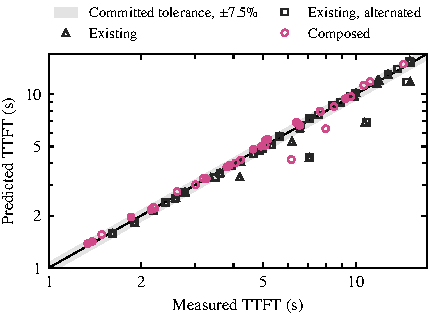
\includegraphics{fig/accuracy.pdf}
    \caption{Predicted against measured TTFT on appends across four LLMs, three schedules, and three splits, with a band of $\pm7.5\%$. The points well below the band are schedules on the one-column attention split, which the event model never chooses, and the existing program on the two-column split at 8{,}192- and 12{,}288-token contexts, which it prices 15--20\% low.}
    \label{fig:accuracy}
\end{figure}

% VALUE: once the order is right a column group, not the CP, binds the lower bound, and which group binds flips with the workload, which is what moves the faster split; the composed schedule lies within a modest factor of the bound, which the event model places closely and never below; no run beats its bound; read as a gap, most of the distance is closed on the dense LLMs and the rest is the overlap's price and unhidden CP and host work
\label{subsec:bound-eval}
Once the order is right, a column group's busy time rather than the CP binds the lower bound, and which group binds flips with the workload.
On Llama-3.2-1B and Qwen3-4B, the GEMMs bind from scratch at 2{,}048 tokens and attention on an append to 16{,}384, at every split, which is why the faster split moves from two attention columns to four (Section~\ref{subsec:split}).
On the twelve appends of Table~\ref{tab:append}, the composed schedule lies $1.17$--$1.63\times$ above the bound, and none of the 33 runs that test the bound ran faster than it (Appendix~\ref{subsec:tests}).
Read as a gap, the schedule closes a median 65\% of the distance from the alternated baseline to the bound, and 34--76\% across these appends, most on the dense LLMs and least on Gemma3-4B, whose windowed attention leaves the GEMMs binding.
What remains is the price of overlap under the DRAM read cap, 1.0--5.1\% of TTFT where the GEMMs bind, and the CP's and the host's work that the schedule does not hide.
% SOURCE: computed in aie-cosched-paper-0 tmp/regime/cells.py over the 24 committed bound cells (2 models x 3 splits x 4 configurations, vault lab-split-sweep (8) / ch3-formulation G6): the binding term is the GEMMs in 12 cells and attention in 12; 1B at 2,048 from scratch the GEMM term rises 377 / 413 / 564 ms from S1 to S4, and on a 16,384 + 4,096 append attention falls 10,776 / 5,258 / 2,631 ms.
% SOURCE: re-derived from amd-npu 78ec55b7 score-2026-10-21.json and checked against Table append (composed / bound = 1.166-1.631; the earlier SOURCE here read 1.196, which is the 1B 2k + 4k cell, not the minimum): predicted minus measured over all 12 is +0.000 to +0.088, median 0.025, never negative; B1 0 violations over 33 runs, the lowest ratio 1.023 (vault lab-split-sweep (27)).
% SOURCE: gap captured, per cell: baseline = the faster of the shipped arms over the three splits, ours = the faster composed arm, floor = the smallest lower bound over the three splits, captured = (baseline - ours) / (baseline - floor). Llama-3.2-1B 70 / 72 / 43%, Qwen3-4B 71 / 75 / 46%, Gemma3-4B 55 / 44 / 34%, Llama-3.1-8B 76 / 73 / 61% at 2k+4k / 8k+4k / 12k+2k; median 65%; the dense LLMs 70-76% on six of their nine cells.
% SOURCE: applying 0.085 x the co-runner where the GEMMs bind gives 6.4-269.2 ms, 1.0-5.1% of TTFT, tightening the gap to the bound from a median 1.23 to 1.17 on those cells; the unhidden CP and host residual is 63-264 ms on the 1B's non-anomalous cells and 139-741 ms on Qwen3-4B's (tmp/regime/cells.py, as above).
% COMMENT: two of the 24 cells are already-excluded artifacts, not evidence: the 1B's S1 16,384 + 4,096 cell ran in the intermittent slow state the record does not quote, and Qwen3-4B's S1 16,384 + 4,096 measures 0.98 of its own bound, which lab-split-sweep (8) records as the bound not being strict where attention is extrapolated tenfold.
% DECISION: the ratio to the bound is the bound at the composed schedule's own split, as Table append reports it; the gap fraction uses the smallest bound over the splits and the stronger baseline, the conservative reading of both.

% VALUE: three hand-written designs put each class of the two cells that hold no costly instance on the critical path and test the textbook condition directly: a removal off the binding cycle is worth nothing, the set that cuts it pays, and a class pays only where it binds
\label{subsec:synthetic}
Three small designs of our own put the two remaining cells of Table~\ref{tab:grid} on the critical path.
Where two name dependences close one cycle through a core, removing either alone gains nothing measurable, whereas removing both gains up to $1.60\times$.
An order dependence inside a loop gains $2.00\times$ where it closes the producer--consumer cycle, and nothing where each core's own loop binds instead.
Each outcome follows from whether the removal cuts the binding cycle (Appendix~\ref{app:synthetic}).
% SOURCE: re-derived from the committed scores (amd-npu 2ea67242 and c4f9a19d, runs-2026-10-22/{aon,ns,ol}/score.json; designs c423a98b, 9c94988a, ea3316e4; all three holds rc 0, no faults, every per-tile output check true). s1 by level, g(2,1) / g(1,2) / g(2,2): m256p1 1.0096 / 1.0031 / 1.5970; m1024p1 1.0003 / 0.9980 / 1.1458; m1024p4 0.9824 / 0.9876 / 1.0312. s2: single-indep 59.21, ring-indep 58.45 ms, g 1.0130, repetition spread 1.5-2.0%. s3: stream-s2 3.610, pair-s2 7.235, stream-s4 11.653, pair-s4 11.643 ms, g 2.0044 and 0.9991 (vault lab-synthetic-classes (4)-(6)). The 1.60x rests on a depth-one baseline whose repetitions span 193% of their median (Appendix synthetic).
% DECISION: no design, depth, or work level was changed after its own measurement, since a design altered after it ran stops being evidence for its class; the slow-side single removals at the third work level are stated with their sizes.

\subsection{Fidelity and Reach}
\label{subsec:fidelity}

% VALUE: the method reads exactly what each stack dispatches: 625 streams of three toolchains re-emit byte for byte, and nearly every wait in 792 streams is attributed to a mechanism, with the residual located; the three stream counts (625 round trip, 792 analysed, 277 in the census) related once, by scope
Because the method starts from streams a stack has already emitted, it must read them exactly, and it does so on all three toolchains.
Re-emitting 625 streams byte for byte shows that the analysis starts from exactly what each stack dispatches, namely 375 streams built by MLIR-AIR and 218 recorded from FastFlowLM, both through the lifter of Section~\ref{subsec:closed}, and 32 built by IRON through IRON's own translator.
Over 792 streams, the analysis attributes 73{,}994 of 74{,}010 waits to one of its ordering mechanisms.
% SOURCE: recording libhrx (FastFlowLM 44d01787, gemma4e-flash), every prompt length 1-1,024 recorded with 0 /dev/accel opens; 8 buckets, 218 distinct streams, round trip and identity 218 / 218 (vault lab-cosched-passes (14)); lifter fix mlir-aie 91f64387ffb, 375 / 375 MLIR-AIR streams byte-identical (lab-cosched-passes (3)); IRON 32 / 32 through its own translator (1-intro SOURCE). Further populations not counted here are in Appendix roundtrip.
% SOURCE: aie-cosched results/2026-10-23-s35-data, registered c57b708, result ef6733a (aie-cosched-stream-deps at mlir-aie 0489d325082): waits 74,010, attributed 73,994; unattributed waits 16 (4 in each of the 4 MLIR-AIR fused-decode streams) and unattributed ops 67 (66 there, 1 IRON); per population AIR 10,256 / 10,240, FLM 63,392 / 63,392, IRON 362 / 362; one IRON stream (179,576 ops) not analysed; 792 streams read.
% SOURCE: 792 = 543 MLIR-AIR + 218 FastFlowLM + 31 IRON analysed streams (aie-cosched 93f491b, mlir-aie f9ad95dc02f, lab-cosched-passes (62), P7c; 4-method Textbook Classes SOURCE); 277 = 27 MLIR-AIR + 32 IRON + 218 FastFlowLM (lab-cosched-passes (41)); 625 = 375 + 218 + 32 (lab-cosched-passes (3), (9), (14)).
% DECISION: the attribution counters are the analysis's edge-level coverage; they are a different quantity from the census's instance count, and the two must not be conflated in the text.

% VALUE: the census: at stream granularity our stream pass, run over 277 streams of three stacks with the known instances excluded, removes no further instance; the zero describes the pass's lane rule (a lane defined), not the streams; the residual bookkeeping is in the appendix
\label{subsec:census}
Beyond the instances of Table~\ref{tab:grid}, the stream pass proposes moves on 29 of 277 streams of the three stacks, and its checker and an independent second implementation (Section~\ref{subsec:checkers}) agree on every verdict, refusing FastFlowLM's 16, which would overflow a channel's task queue, and accepting IRON's 13.
% SOURCE: population 277 = 27 MLIR-AIR + 32 IRON + 218 FastFlowLM (vault lab-cosched-passes (41) and its addendum). aie-cosched tools/oracle_results/2026-10-21-d3 prex_scan.json: monotone proposals 0 on all 277; full-mode moves on 29 (16 FastFlowLM wait-free-lane hoists, 13 IRON in-block moves) (foundation audit 2026-10-22, Phase 2.B J7).
% SOURCE: aie-cosched 9912aa9 (lab-cosched-passes (62), the iron13 run): the 13 IRON moves ACCEPTED by the C++ checker and legality.check on each stream's own configuration (3 binary_elementwise on their xclbin and routed device; 10 decode-fused_op on the device whose runtime sequence has the stream's skeleton), none crossing a wait; worth unpriced.
% SOURCE: aie-cosched baf37e0 (lab-cosched-passes (62), P7b): lanes.json byte-equal to the reviewer's 8da59d9a (247 / 29 / 1 streams with 1 / 2 / 0 lanes); the 16 two-lane production-engine streams REFUSED on all 16 by legality.check (full, configured) and the C++ checker with identical decided codes: QUEUE-OVERFLOW on the 8 of columns 0/3, QUEUE-OVERFLOW + FENCE-CROSSED-UNPROVEN on the 8 of columns 6/7, no BD-REUSE.
% SOURCE: the lane rule is (35). Breakdown: 199 single-lane by the lane rule (193 production + 6 IRON gemm + 1 other), 61 single-phase (60 issuing nothing after the first wait, plus IRON decode-fused_op fc078b33, 179,576 ops, unplaced), 16 with queue overflow. The characterization is B-prime (vault (46)): 193 of 218 with at least one accepted reordering at 1.000-1.0069, IRON 0 of 84 accepted (all queue-overflow), MLIR-AIR none proposed.
% DECISION: the census reports the pass's proposals and verdicts, not a census zero; at loop granularity the text states what the analysis judges.
% DECISION: the census() procedure as first specified is NOT-READY on the committed artifacts (its pre-scan commit was never made); the text reports the pass's offline steps, which ran with the same pass and checkers, and never calls the zero the result of that procedure.

% VALUE: at loop granularity the analysis judges every loop of the MLIR-AIR designs and part of IRON's, with the reason for the rest; our passes judge MLIR-AIR designs of LLMs never examined, with no gain claimed; the reach differs by what each toolchain exposes
At loop granularity, the analysis judges all 3{,}719 loops of the MLIR-AIR prefill and decode designs, and 50 of IRON's 242, whose others hold a lock across an inner loop with a trip count the dispatch does not give.
Our passes also judge the MLIR-AIR designs of five LLMs we never ran or examined, Llama-3.2-3B, Phi-4-mini, Qwen2.5-3B and~7B, and Qwen3-8B.
On their decodes the loop pass renames attention's keys, values, and scores as on the evaluated LLMs and finds every other loop's buffers already multi-slot, and on three of their prefills it judges every loop, but we claim no gain on any of them.
The method's reach thus follows what each toolchain exposes, since we read and rewrite MLIR-AIR's designs, read and check IRON's, and read and classify FastFlowLM's (Section~\ref{subsec:closed}).
% SOURCE: aie-cosched results/2026-10-23-s35-data, registered c57b708, result 3dbc1ee (mlir-aie dev 027651259b5): MLIR-AIR prefill 3,488 / 3,488 judged over 109 designs (1,184 single-slot renamable), the nine fused decodes 231 / 231 (102), IRON 50 / 242 (192 refused: an inner lock-holding loop whose trip count is not derivable from the dispatch).
% SOURCE: P8 (a), the unexamined MLIR-AIR models (aie-cosched e5ad472; expectations committed before the runs; 0 accel opens; kernels byte-identical): 5 decodes (Llama-3.2-3B, Phi-4-mini, Qwen2.5-7B / 3B, Qwen3-8B), the attention ring renamed, 12 buffers (6 on Qwen2.5-3B); 3 prefills (Llama-3.2-3B, Phi-4-mini, Qwen3-8B), every loop judged, single-slot renamable buffers only the GEMM output tiles, 168 / 168 / 144, worth unpriced. Ruling 3 (registered 7687182, results/2026-10-23-phase-rerun; mlir-aie 0c5e8e37fac / 6b9e6666991, lit 46/46): on all nine fused decodes every loop is judged, 0 refused, and the projection loops' name buffers are all multi-slot already (vault decisions log, P8 (a) and Ruling 3).
% SOURCE: FastFlowLM's closed libraries build its streams and buffers, so removals are measured on MLIR-AIR's fused prefill, which reimplements FastFlowLM's designs (mlir-air llms README; Section~\ref{subsec:closed}).
% DECISION: the designs never examined are judged by the passes, never credited with a gain (contract, "No overclaim"); no device run exists for them.

\subsection{Overheads}
\label{subsec:overheads}

% VALUE: OPCORD's own costs are one-time per prompt shape or per LLM and split, outside the measured call except a small binding step that every TTFT includes; even charged per request the composed schedule stays ahead of the existing program on the two-column split (a different baseline, named); memory and switching costs are priced in the appendix
OPCORD's costs are paid once per prompt shape, LLM, and split, and they stay below its gains even when charged on every request.
On the two-column split, composing a shape's commands takes 56--148\,ms on Llama-3.2-1B and 143--368\,ms on Qwen3-4B, and planning it 63--206\,ms and 0.3--1.1\,s; later prompts of that shape reuse this work, whereas an agent's turn, whose cached context grows, pays it each time.
Charged on every request, the composed schedule still leads the existing program on that split by $1.13$--$2.18\times$ at every configuration we measure.
Every TTFT includes the 7--50\,ms that binding attention's positions takes inside the call.
Probing each operator alone costs 9--39\,s, paid once per LLM and split.
Appendices~\ref{app:rings} and~\ref{app:relayout} price the memory and the switches between splits.
% SOURCE: composition measured host-only before and after the operator-level cache (amd-npu 82c5b5b0, compose-gate-2026-10-22/; stand-in pyxrt). Gate: 56 cells over 5 models and 14 builds, 65,550 commands and 325,974,776 words, every command byte-identical to the previous path, so every device measurement we hold is unaffected. S2 composition: 1B 56 / 148 / 140 / 128 ms; Qwen 143 / 368 / 240 / 297 ms at scratch 2k / scratch 4k / 4k+4k / 16k+4k. Per-request bound against the run medians and the shipped arm's own first-call extra: 1B 1.18 / 1.31 / 1.64 / 2.18, Qwen 1.13 / 1.26 / 1.53 / 1.51. The shipped arm's own per-call composition, from its first call against its later ones, is -80 to +87 ms (Appendix overheads).
% SOURCE: planning 63-206 ms (1B) and 0.3-1.1 s (Qwen3-4B); bind step 7-14 ms (1B) and 15-50 ms (larger models); probes 9-39 s per model and split (vault lab-split-sweep (29)-(30)).
% DECISION: planning is the larger one-time term and is left as it is; it makes no cell a loss, and the paper does not claim the prototype is fast, only that its cost is one-time and bounded.
% DECISION: Table 2 (overheads) stays dropped. Four of its five rows restate numbers stated beside the design decision they price, and the fifth, planning time, is answered here.
% COMMENT: the planning VERIFY that stood here is answered for the two-column split (lab-split-sweep (29)-(30)). Open (foundation audit 2026-10-22, B37): the per-request charge is not computed on the four-column split the composer takes for appends, where composition alone is 131-214 ms (1B) and 236-567 ms (Qwen3-4B).
